\documentclass[11pt]{article}
\usepackage[textwidth=18.0cm, textheight=23.0cm, top=2.0cm]{geometry}
\usepackage{pst-all}
\usepackage{amssymb}
\usepackage{tikz}
\usepackage{underscore}\begin{document}
\pagestyle{empty}


ClassName: \underline{\textbf{Class_10.2bp-33}}
\par
BinSize: \underline{\textbf{100 × 100}}
\par
ReduceSize: \underline{\textbf{100 × 100}}
\par
TypeNum: \underline{\textbf{79}}
\par
Num: \underline{\textbf{80}}
\par
OutS: \underline{\textbf{140000}}
\par
InS: \underline{\textbf{129404}}
\par
Rate: \underline{\textbf{0.924}}
\par
UB: \underline{\textbf{14}}
\par
LB0: \underline{\textbf{14}}
\par
LB: \underline{\textbf{14}}
\par
LBWithCut: \underline{\textbf{14}}
\par
NodeCut: \underline{\textbf{0}}
\par
ExtendedNodeCnt: \underline{\textbf{1}}
\par
GenNodeCnt: \underline{\textbf{1}}
\par
PrimalNode: \underline{\textbf{0}}
\par
ColumnCount: \underline{\textbf{14}}
\par
TotalCutCount: \underline{\textbf{0}}
\par
RootCutCount: \underline{\textbf{0}}
\par
LPSolverCnt: \underline{\textbf{1}}
\par
PricingSolverCnt: \underline{\textbf{0}}
\par
BranchAndBoundNum: \underline{\textbf{1}}
\par
isOpt: \underline{\textbf{true}}
\par
TimeOnInitSolution: \underline{\textbf{120.020 s}}
\par
TimeOnPrimal: \underline{\textbf{0.000 s}}
\par
TimeOnPricing: \underline{\textbf{0.000 s}}
\par
TimeOnRmp: \underline{\textbf{0.078 s}}
\par
TotalTime: \underline{\textbf{120.160 s}}
\par
\newpage


\begin{tikzpicture}[shorten >=1pt,scale=1.0,every node/.style={scale=1.0},->]
\tikzstyle{vertex}=[circle,fill=black!25,minimum size=14pt,inner sep=0pt]
\filldraw[fill=gray!40!white, draw=black] (0,0) rectangle (15.0,15.0);
\foreach \name/\x/\y/\w/\h in {90x100/0.0/0.0/13.5/15.0,10x47/13.5/0.0/1.5/7.05,9x47/13.5/7.6499999999999995/1.3499999999999999/7.05,10x4/13.5/7.05/1.5/0.6}
\filldraw[fill=white!40!white, draw=black] (\x,\y) rectangle node[draw] (\name) {\name} ++(\w,\h);
\end{tikzpicture}


w =90 , h =100 , x =0 , y =0 , v =9000
\par
w =10 , h =47 , x =90 , y =0 , v =470
\par
w =9 , h =47 , x =90 , y =51 , v =423
\par
w =10 , h =4 , x =90 , y =47 , v =40
\par
\newpage


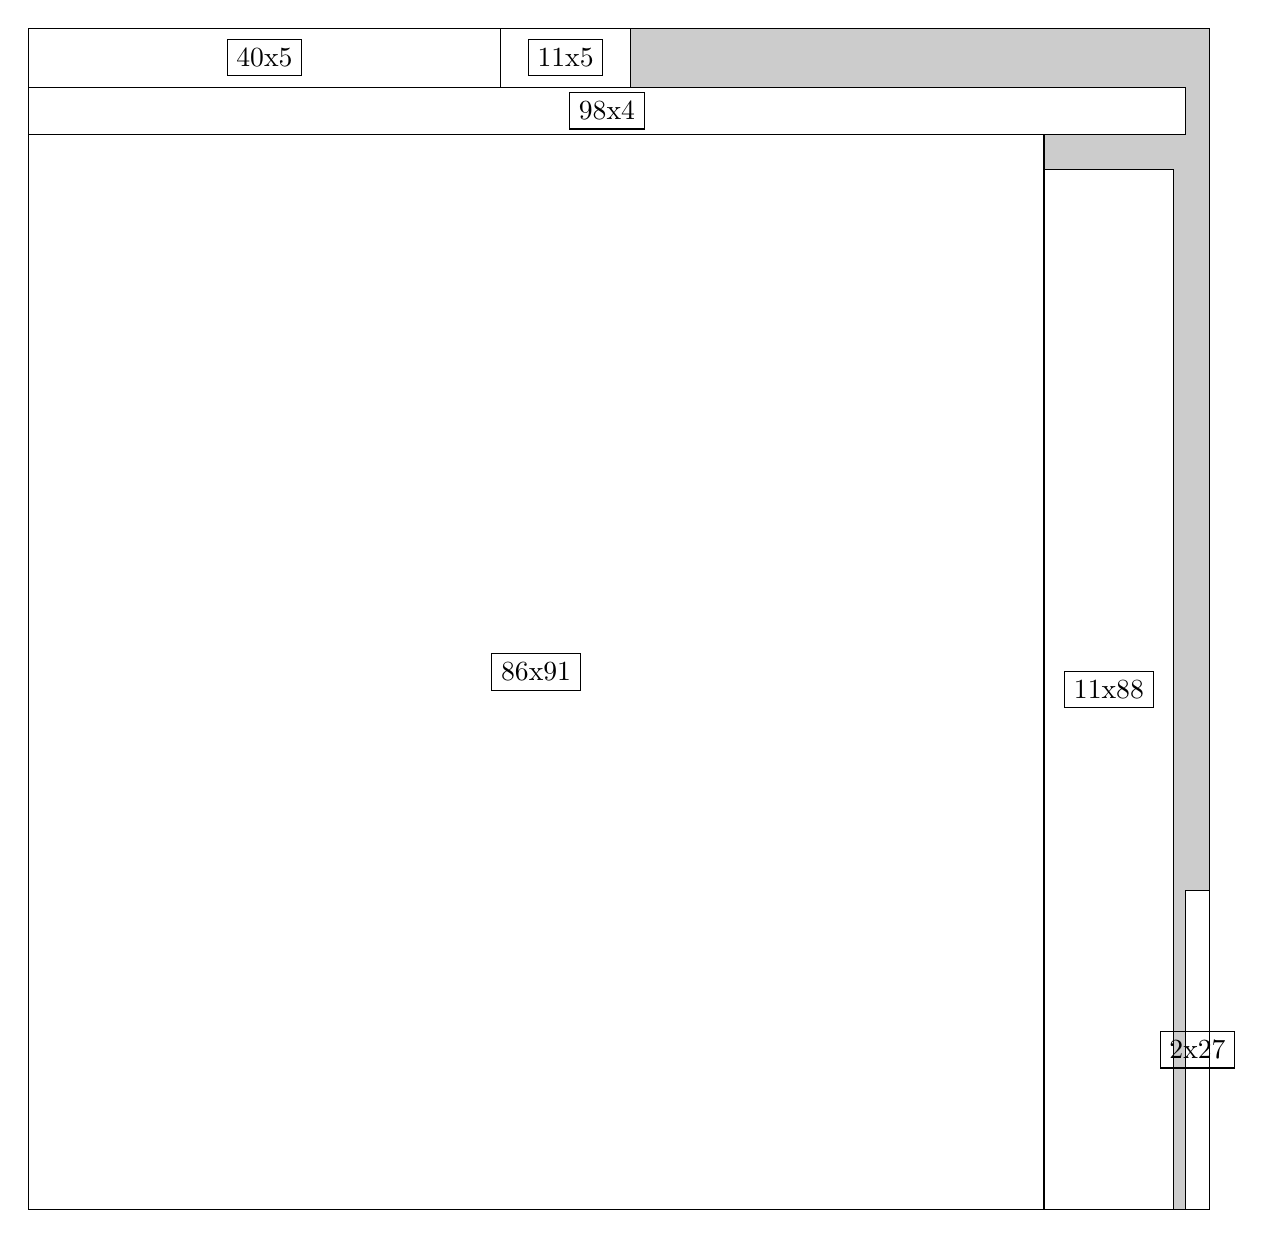
\begin{tikzpicture}[shorten >=1pt,scale=1.0,every node/.style={scale=1.0},->]
\tikzstyle{vertex}=[circle,fill=black!25,minimum size=14pt,inner sep=0pt]
\filldraw[fill=gray!40!white, draw=black] (0,0) rectangle (15.0,15.0);
\foreach \name/\x/\y/\w/\h in {86x91/0.0/0.0/12.9/13.65,11x88/12.9/0.0/1.65/13.2,98x4/0.0/13.65/14.7/0.6,40x5/0.0/14.25/6.0/0.75,11x5/6.0/14.25/1.65/0.75,2x27/14.7/0.0/0.3/4.05}
\filldraw[fill=white!40!white, draw=black] (\x,\y) rectangle node[draw] (\name) {\name} ++(\w,\h);
\end{tikzpicture}


w =86 , h =91 , x =0 , y =0 , v =7826
\par
w =11 , h =88 , x =86 , y =0 , v =968
\par
w =98 , h =4 , x =0 , y =91 , v =392
\par
w =40 , h =5 , x =0 , y =95 , v =200
\par
w =11 , h =5 , x =40 , y =95 , v =55
\par
w =2 , h =27 , x =98 , y =0 , v =54
\par
\newpage


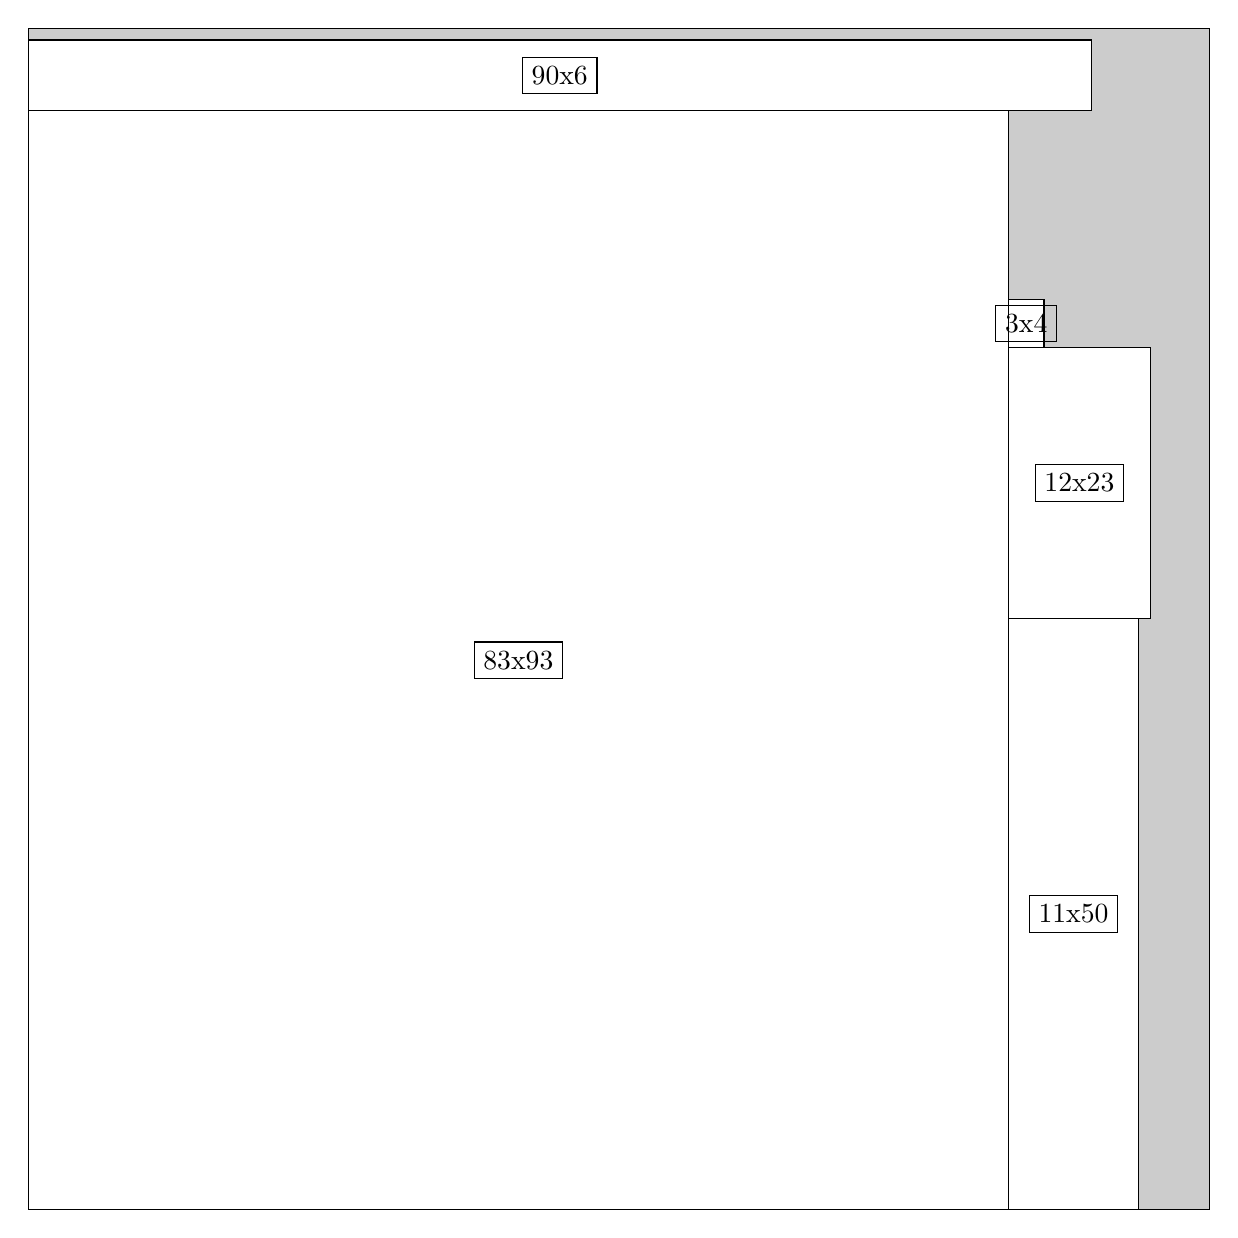
\begin{tikzpicture}[shorten >=1pt,scale=1.0,every node/.style={scale=1.0},->]
\tikzstyle{vertex}=[circle,fill=black!25,minimum size=14pt,inner sep=0pt]
\filldraw[fill=gray!40!white, draw=black] (0,0) rectangle (15.0,15.0);
\foreach \name/\x/\y/\w/\h in {83x93/0.0/0.0/12.45/13.95,11x50/12.45/0.0/1.65/7.5,90x6/0.0/13.95/13.5/0.8999999999999999,12x23/12.45/7.5/1.7999999999999998/3.4499999999999997,3x4/12.45/10.95/0.44999999999999996/0.6}
\filldraw[fill=white!40!white, draw=black] (\x,\y) rectangle node[draw] (\name) {\name} ++(\w,\h);
\end{tikzpicture}


w =83 , h =93 , x =0 , y =0 , v =7719
\par
w =11 , h =50 , x =83 , y =0 , v =550
\par
w =90 , h =6 , x =0 , y =93 , v =540
\par
w =12 , h =23 , x =83 , y =50 , v =276
\par
w =3 , h =4 , x =83 , y =73 , v =12
\par
\newpage


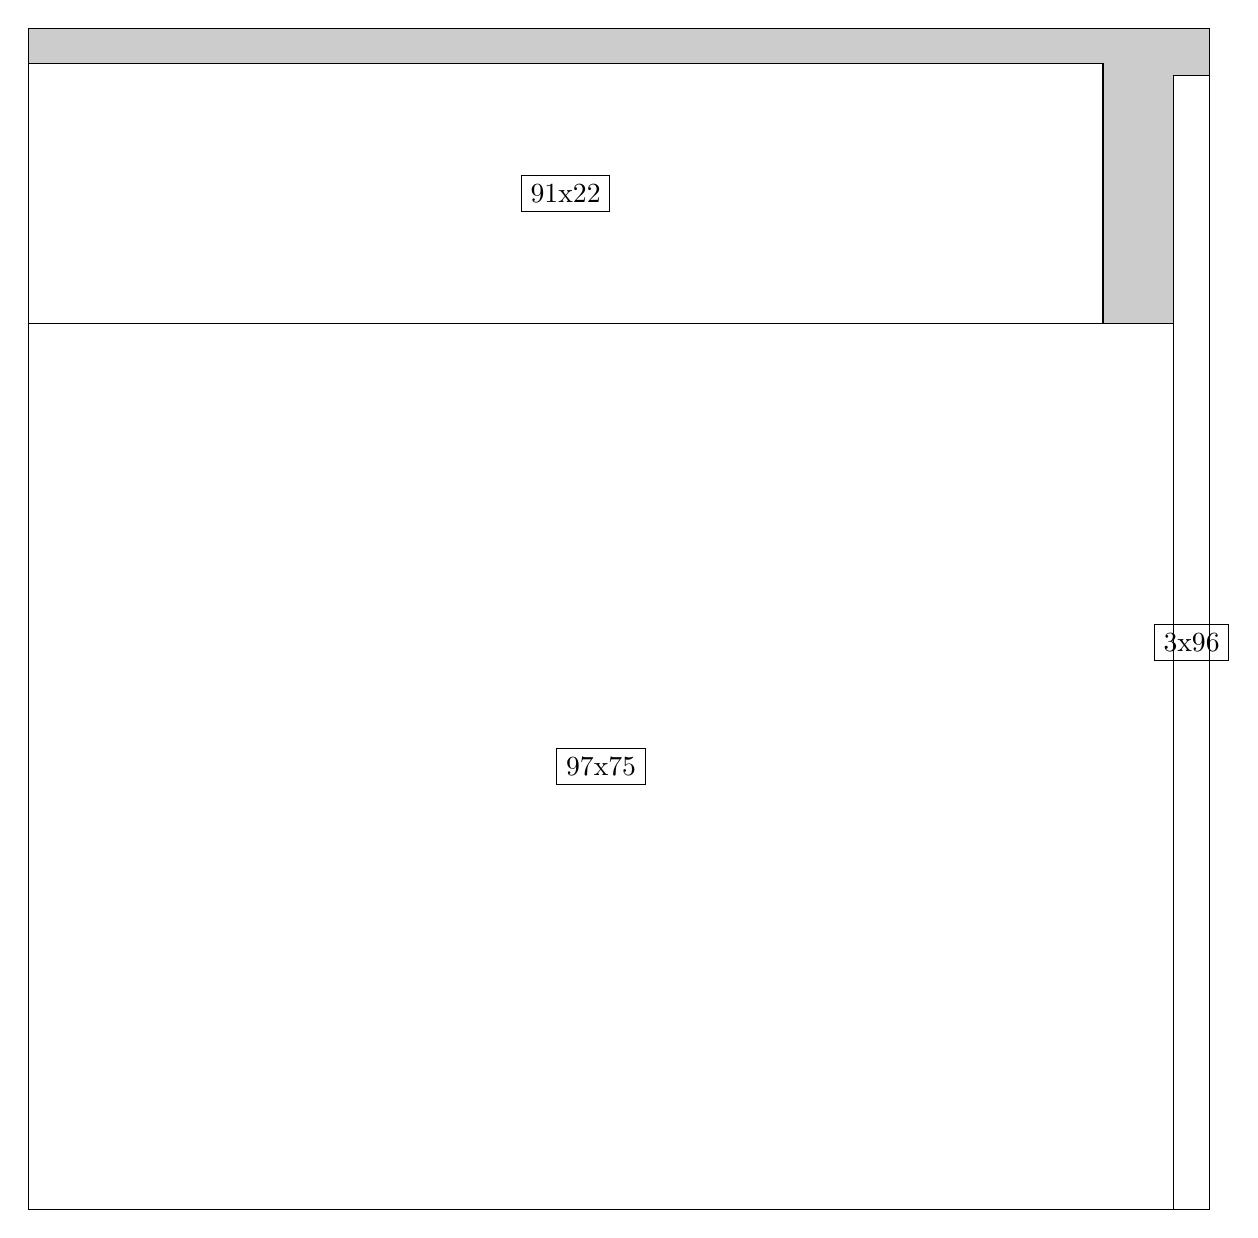
\begin{tikzpicture}[shorten >=1pt,scale=1.0,every node/.style={scale=1.0},->]
\tikzstyle{vertex}=[circle,fill=black!25,minimum size=14pt,inner sep=0pt]
\filldraw[fill=gray!40!white, draw=black] (0,0) rectangle (15.0,15.0);
\foreach \name/\x/\y/\w/\h in {97x75/0.0/0.0/14.549999999999999/11.25,91x22/0.0/11.25/13.65/3.3,3x96/14.549999999999999/0.0/0.44999999999999996/14.399999999999999}
\filldraw[fill=white!40!white, draw=black] (\x,\y) rectangle node[draw] (\name) {\name} ++(\w,\h);
\end{tikzpicture}


w =97 , h =75 , x =0 , y =0 , v =7275
\par
w =91 , h =22 , x =0 , y =75 , v =2002
\par
w =3 , h =96 , x =97 , y =0 , v =288
\par
\newpage


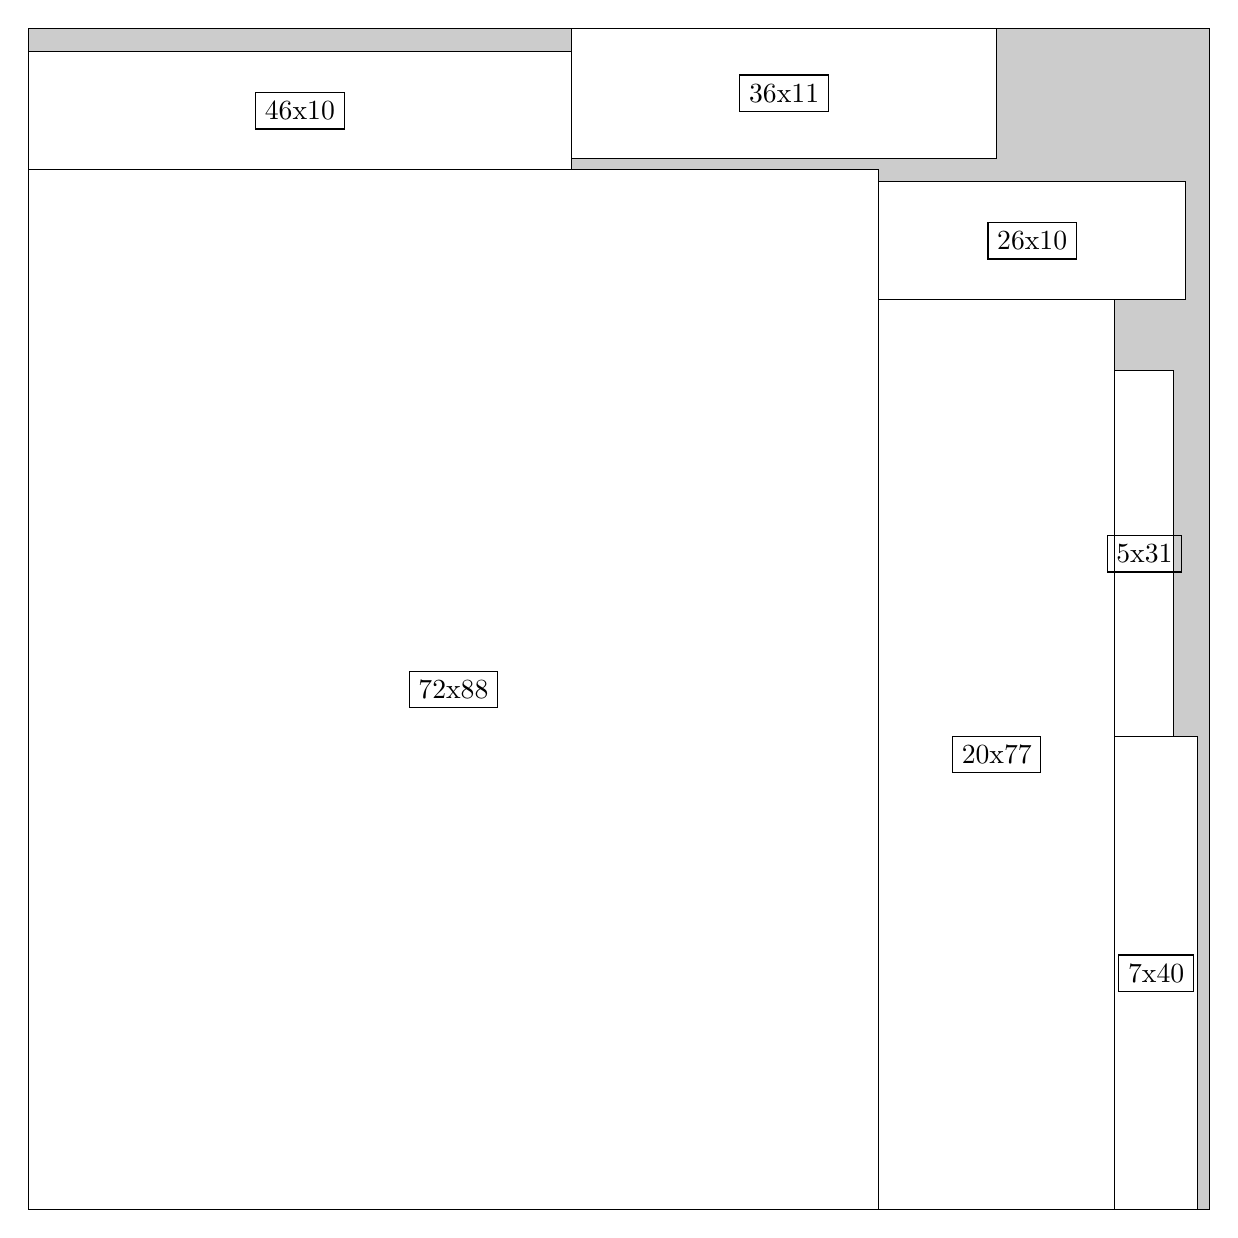
\begin{tikzpicture}[shorten >=1pt,scale=1.0,every node/.style={scale=1.0},->]
\tikzstyle{vertex}=[circle,fill=black!25,minimum size=14pt,inner sep=0pt]
\filldraw[fill=gray!40!white, draw=black] (0,0) rectangle (15.0,15.0);
\foreach \name/\x/\y/\w/\h in {72x88/0.0/0.0/10.799999999999999/13.2,20x77/10.799999999999999/0.0/3.0/11.549999999999999,46x10/0.0/13.2/6.8999999999999995/1.5,36x11/6.8999999999999995/13.35/5.3999999999999995/1.65,7x40/13.799999999999999/0.0/1.05/6.0,26x10/10.799999999999999/11.549999999999999/3.9/1.5,5x31/13.799999999999999/6.0/0.75/4.6499999999999995}
\filldraw[fill=white!40!white, draw=black] (\x,\y) rectangle node[draw] (\name) {\name} ++(\w,\h);
\end{tikzpicture}


w =72 , h =88 , x =0 , y =0 , v =6336
\par
w =20 , h =77 , x =72 , y =0 , v =1540
\par
w =46 , h =10 , x =0 , y =88 , v =460
\par
w =36 , h =11 , x =46 , y =89 , v =396
\par
w =7 , h =40 , x =92 , y =0 , v =280
\par
w =26 , h =10 , x =72 , y =77 , v =260
\par
w =5 , h =31 , x =92 , y =40 , v =155
\par
\newpage


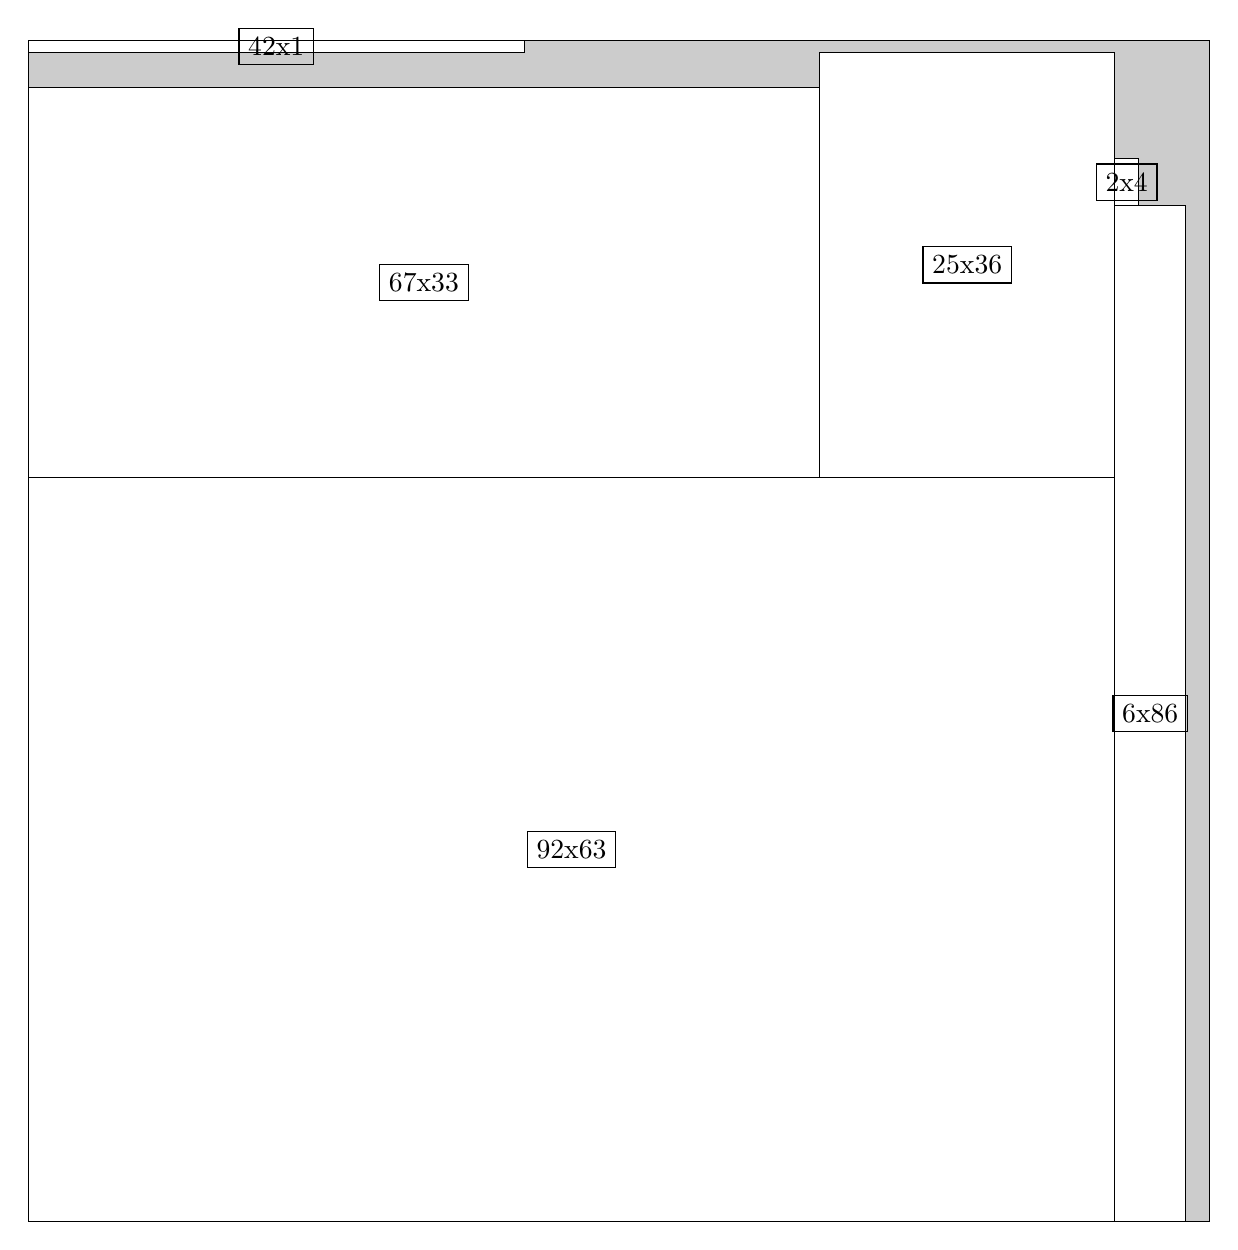
\begin{tikzpicture}[shorten >=1pt,scale=1.0,every node/.style={scale=1.0},->]
\tikzstyle{vertex}=[circle,fill=black!25,minimum size=14pt,inner sep=0pt]
\filldraw[fill=gray!40!white, draw=black] (0,0) rectangle (15.0,15.0);
\foreach \name/\x/\y/\w/\h in {92x63/0.0/0.0/13.799999999999999/9.45,67x33/0.0/9.45/10.049999999999999/4.95,25x36/10.049999999999999/9.45/3.75/5.3999999999999995,6x86/13.799999999999999/0.0/0.8999999999999999/12.9,42x1/0.0/14.85/6.3/0.15,2x4/13.799999999999999/12.9/0.3/0.6}
\filldraw[fill=white!40!white, draw=black] (\x,\y) rectangle node[draw] (\name) {\name} ++(\w,\h);
\end{tikzpicture}


w =92 , h =63 , x =0 , y =0 , v =5796
\par
w =67 , h =33 , x =0 , y =63 , v =2211
\par
w =25 , h =36 , x =67 , y =63 , v =900
\par
w =6 , h =86 , x =92 , y =0 , v =516
\par
w =42 , h =1 , x =0 , y =99 , v =42
\par
w =2 , h =4 , x =92 , y =86 , v =8
\par
\newpage


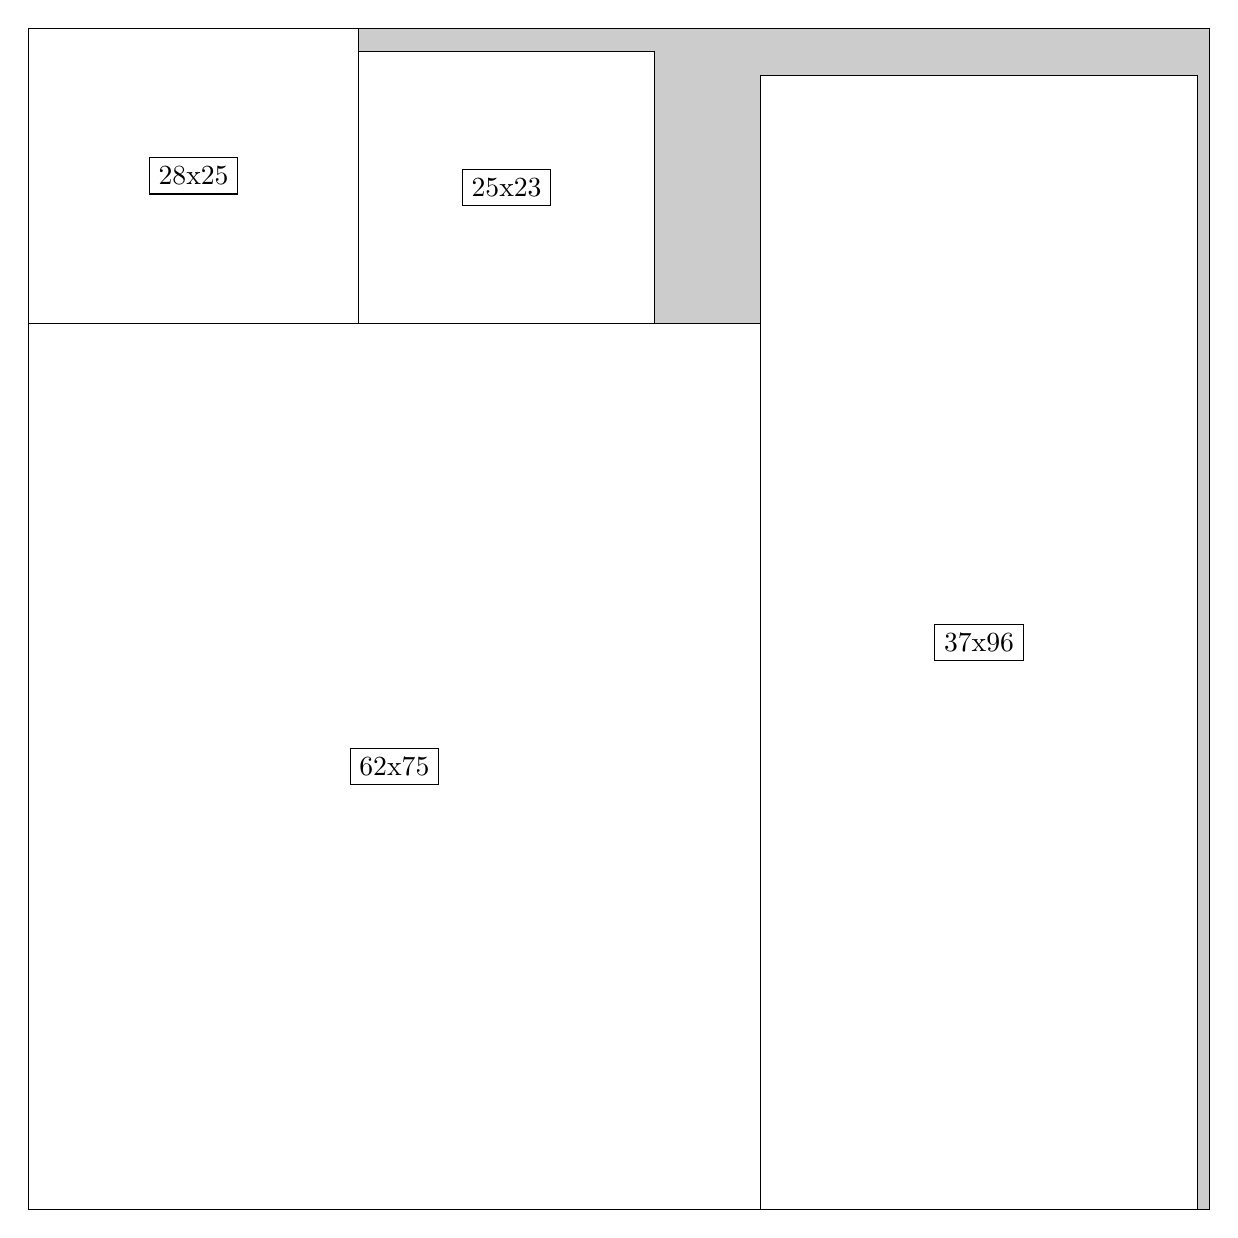
\begin{tikzpicture}[shorten >=1pt,scale=1.0,every node/.style={scale=1.0},->]
\tikzstyle{vertex}=[circle,fill=black!25,minimum size=14pt,inner sep=0pt]
\filldraw[fill=gray!40!white, draw=black] (0,0) rectangle (15.0,15.0);
\foreach \name/\x/\y/\w/\h in {62x75/0.0/0.0/9.299999999999999/11.25,37x96/9.299999999999999/0.0/5.55/14.399999999999999,28x25/0.0/11.25/4.2/3.75,25x23/4.2/11.25/3.75/3.4499999999999997}
\filldraw[fill=white!40!white, draw=black] (\x,\y) rectangle node[draw] (\name) {\name} ++(\w,\h);
\end{tikzpicture}


w =62 , h =75 , x =0 , y =0 , v =4650
\par
w =37 , h =96 , x =62 , y =0 , v =3552
\par
w =28 , h =25 , x =0 , y =75 , v =700
\par
w =25 , h =23 , x =28 , y =75 , v =575
\par
\newpage


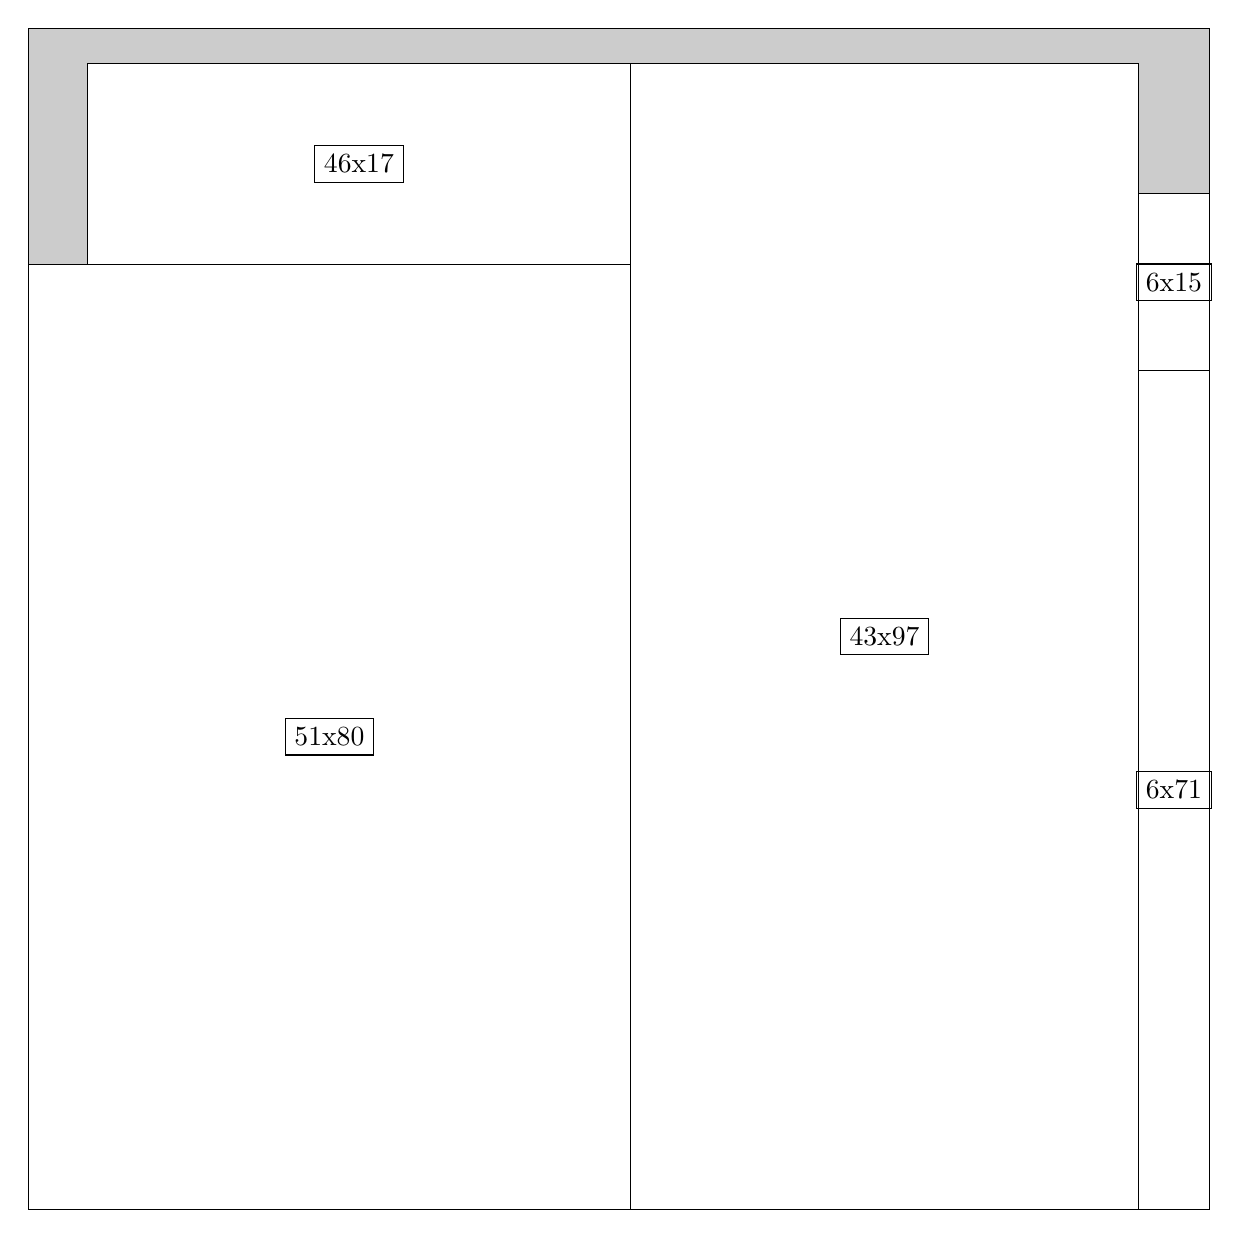
\begin{tikzpicture}[shorten >=1pt,scale=1.0,every node/.style={scale=1.0},->]
\tikzstyle{vertex}=[circle,fill=black!25,minimum size=14pt,inner sep=0pt]
\filldraw[fill=gray!40!white, draw=black] (0,0) rectangle (15.0,15.0);
\foreach \name/\x/\y/\w/\h in {43x97/7.6499999999999995/0.0/6.45/14.549999999999999,51x80/0.0/0.0/7.6499999999999995/12.0,46x17/0.75/12.0/6.8999999999999995/2.55,6x71/14.1/0.0/0.8999999999999999/10.65,6x15/14.1/10.65/0.8999999999999999/2.25}
\filldraw[fill=white!40!white, draw=black] (\x,\y) rectangle node[draw] (\name) {\name} ++(\w,\h);
\end{tikzpicture}


w =43 , h =97 , x =51 , y =0 , v =4171
\par
w =51 , h =80 , x =0 , y =0 , v =4080
\par
w =46 , h =17 , x =5 , y =80 , v =782
\par
w =6 , h =71 , x =94 , y =0 , v =426
\par
w =6 , h =15 , x =94 , y =71 , v =90
\par
\newpage


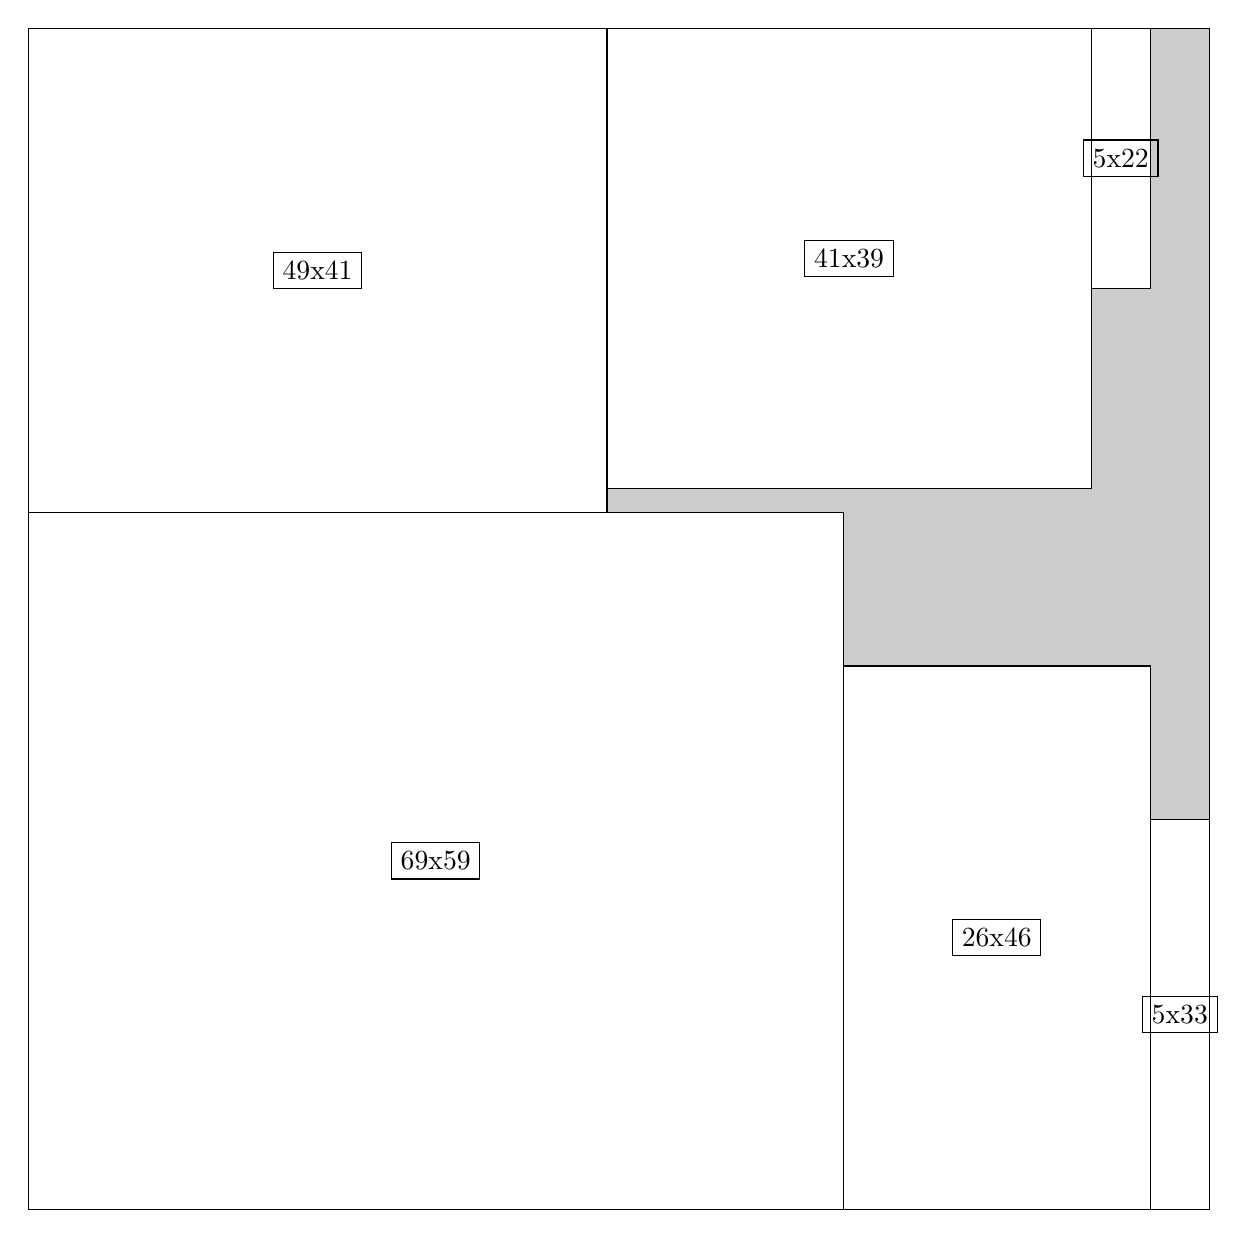
\begin{tikzpicture}[shorten >=1pt,scale=1.0,every node/.style={scale=1.0},->]
\tikzstyle{vertex}=[circle,fill=black!25,minimum size=14pt,inner sep=0pt]
\filldraw[fill=gray!40!white, draw=black] (0,0) rectangle (15.0,15.0);
\foreach \name/\x/\y/\w/\h in {69x59/0.0/0.0/10.35/8.85,49x41/0.0/8.85/7.35/6.1499999999999995,41x39/7.35/9.15/6.1499999999999995/5.85,26x46/10.35/0.0/3.9/6.8999999999999995,5x33/14.25/0.0/0.75/4.95,5x22/13.5/11.7/0.75/3.3}
\filldraw[fill=white!40!white, draw=black] (\x,\y) rectangle node[draw] (\name) {\name} ++(\w,\h);
\end{tikzpicture}


w =69 , h =59 , x =0 , y =0 , v =4071
\par
w =49 , h =41 , x =0 , y =59 , v =2009
\par
w =41 , h =39 , x =49 , y =61 , v =1599
\par
w =26 , h =46 , x =69 , y =0 , v =1196
\par
w =5 , h =33 , x =95 , y =0 , v =165
\par
w =5 , h =22 , x =90 , y =78 , v =110
\par
\newpage


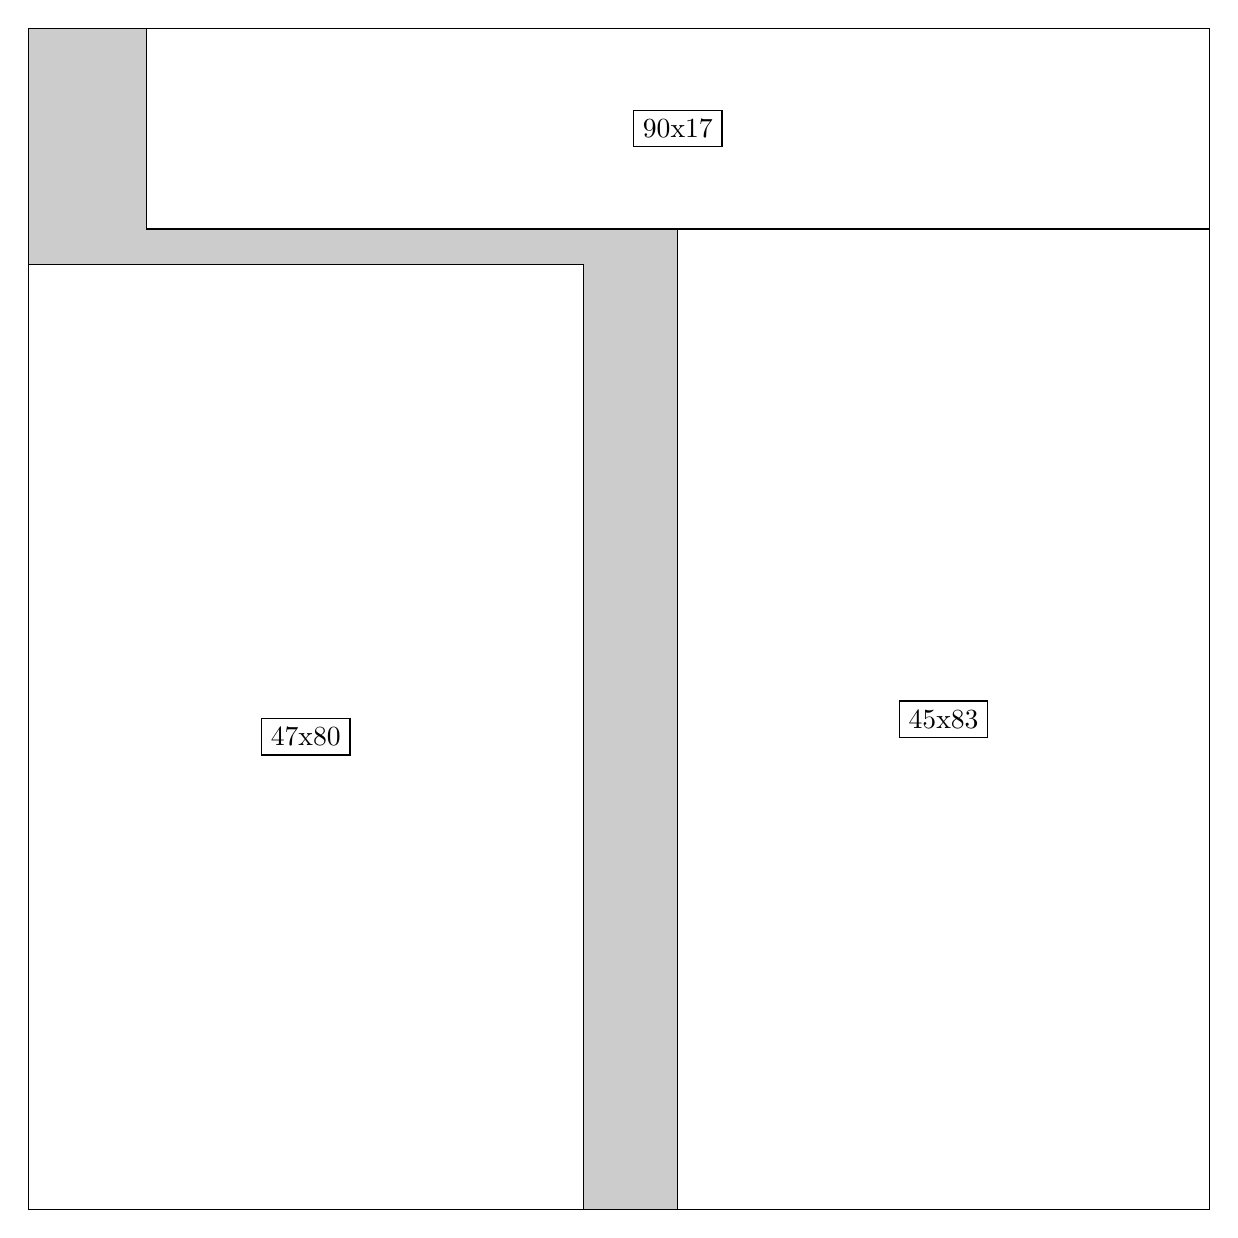
\begin{tikzpicture}[shorten >=1pt,scale=1.0,every node/.style={scale=1.0},->]
\tikzstyle{vertex}=[circle,fill=black!25,minimum size=14pt,inner sep=0pt]
\filldraw[fill=gray!40!white, draw=black] (0,0) rectangle (15.0,15.0);
\foreach \name/\x/\y/\w/\h in {47x80/0.0/0.0/7.05/12.0,45x83/8.25/0.0/6.75/12.45,90x17/1.5/12.45/13.5/2.55}
\filldraw[fill=white!40!white, draw=black] (\x,\y) rectangle node[draw] (\name) {\name} ++(\w,\h);
\end{tikzpicture}


w =47 , h =80 , x =0 , y =0 , v =3760
\par
w =45 , h =83 , x =55 , y =0 , v =3735
\par
w =90 , h =17 , x =10 , y =83 , v =1530
\par
\newpage


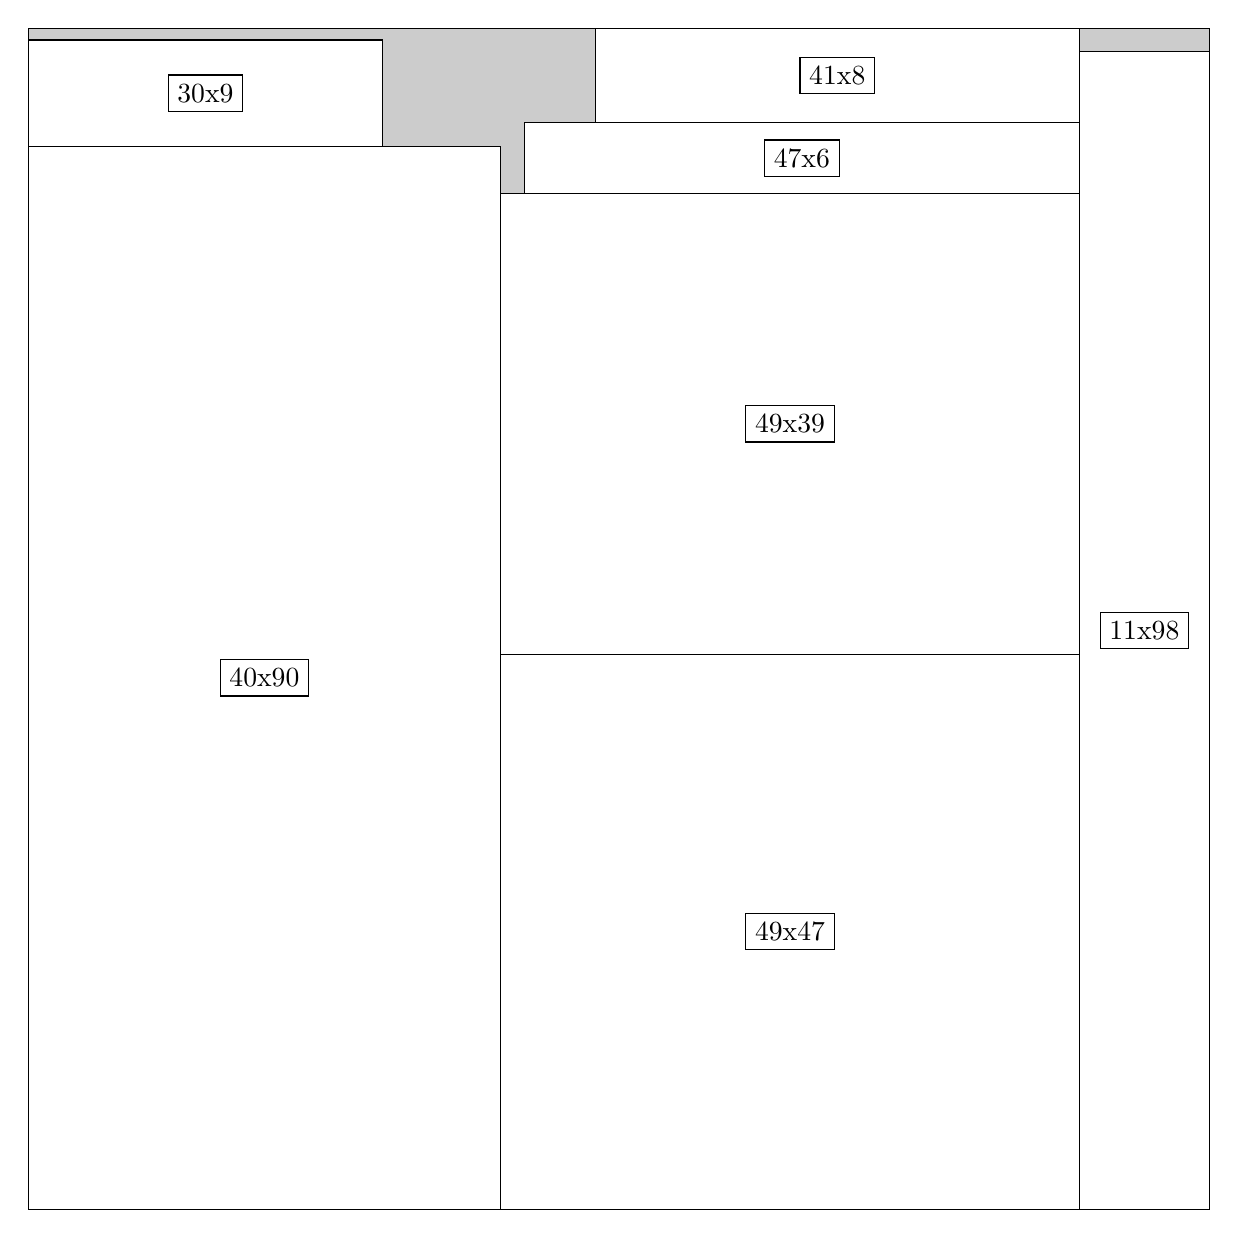
\begin{tikzpicture}[shorten >=1pt,scale=1.0,every node/.style={scale=1.0},->]
\tikzstyle{vertex}=[circle,fill=black!25,minimum size=14pt,inner sep=0pt]
\filldraw[fill=gray!40!white, draw=black] (0,0) rectangle (15.0,15.0);
\foreach \name/\x/\y/\w/\h in {40x90/0.0/0.0/6.0/13.5,11x98/13.35/0.0/1.65/14.7,49x47/6.0/0.0/7.35/7.05,49x39/6.0/7.05/7.35/5.85,41x8/7.199999999999999/13.799999999999999/6.1499999999999995/1.2,47x6/6.3/12.9/7.05/0.8999999999999999,30x9/0.0/13.5/4.5/1.3499999999999999}
\filldraw[fill=white!40!white, draw=black] (\x,\y) rectangle node[draw] (\name) {\name} ++(\w,\h);
\end{tikzpicture}


w =40 , h =90 , x =0 , y =0 , v =3600
\par
w =11 , h =98 , x =89 , y =0 , v =1078
\par
w =49 , h =47 , x =40 , y =0 , v =2303
\par
w =49 , h =39 , x =40 , y =47 , v =1911
\par
w =41 , h =8 , x =48 , y =92 , v =328
\par
w =47 , h =6 , x =42 , y =86 , v =282
\par
w =30 , h =9 , x =0 , y =90 , v =270
\par
\newpage


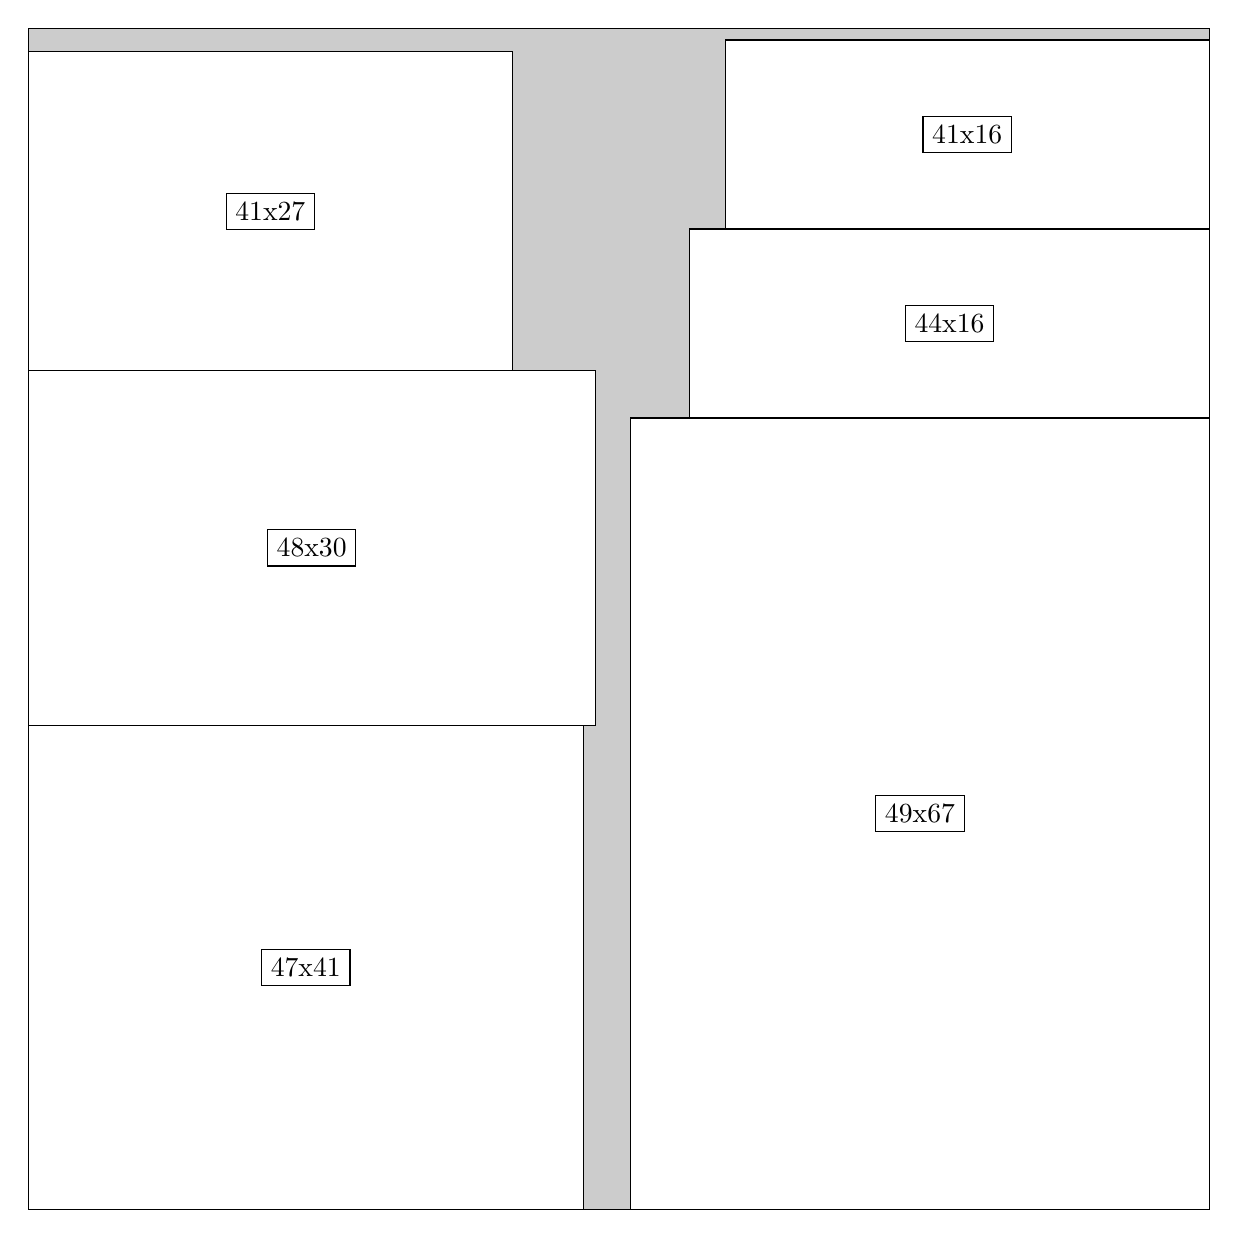
\begin{tikzpicture}[shorten >=1pt,scale=1.0,every node/.style={scale=1.0},->]
\tikzstyle{vertex}=[circle,fill=black!25,minimum size=14pt,inner sep=0pt]
\filldraw[fill=gray!40!white, draw=black] (0,0) rectangle (15.0,15.0);
\foreach \name/\x/\y/\w/\h in {47x41/0.0/0.0/7.05/6.1499999999999995,48x30/0.0/6.1499999999999995/7.199999999999999/4.5,41x27/0.0/10.65/6.1499999999999995/4.05,49x67/7.6499999999999995/0.0/7.35/10.049999999999999,44x16/8.4/10.049999999999999/6.6/2.4,41x16/8.85/12.45/6.1499999999999995/2.4}
\filldraw[fill=white!40!white, draw=black] (\x,\y) rectangle node[draw] (\name) {\name} ++(\w,\h);
\end{tikzpicture}


w =47 , h =41 , x =0 , y =0 , v =1927
\par
w =48 , h =30 , x =0 , y =41 , v =1440
\par
w =41 , h =27 , x =0 , y =71 , v =1107
\par
w =49 , h =67 , x =51 , y =0 , v =3283
\par
w =44 , h =16 , x =56 , y =67 , v =704
\par
w =41 , h =16 , x =59 , y =83 , v =656
\par
\newpage


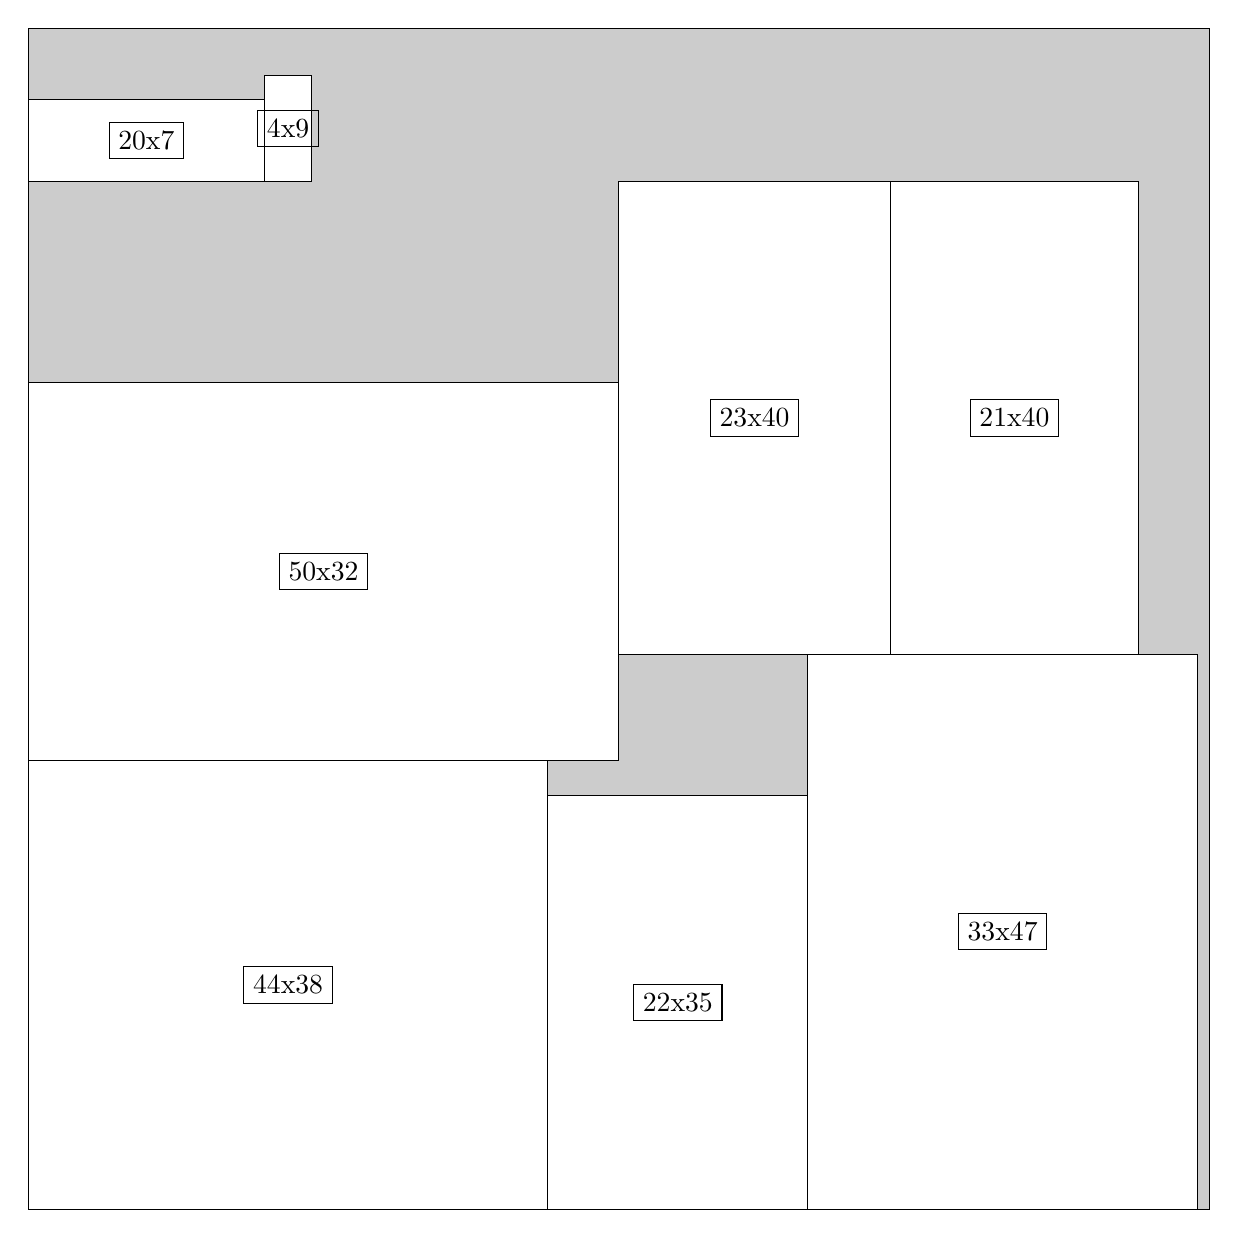
\begin{tikzpicture}[shorten >=1pt,scale=1.0,every node/.style={scale=1.0},->]
\tikzstyle{vertex}=[circle,fill=black!25,minimum size=14pt,inner sep=0pt]
\filldraw[fill=gray!40!white, draw=black] (0,0) rectangle (15.0,15.0);
\foreach \name/\x/\y/\w/\h in {44x38/0.0/0.0/6.6/5.7,50x32/0.0/5.7/7.5/4.8,33x47/9.9/0.0/4.95/7.05,23x40/7.5/7.05/3.4499999999999997/6.0,21x40/10.95/7.05/3.15/6.0,22x35/6.6/0.0/3.3/5.25,20x7/0.0/13.049999999999999/3.0/1.05,4x9/3.0/13.049999999999999/0.6/1.3499999999999999}
\filldraw[fill=white!40!white, draw=black] (\x,\y) rectangle node[draw] (\name) {\name} ++(\w,\h);
\end{tikzpicture}


w =44 , h =38 , x =0 , y =0 , v =1672
\par
w =50 , h =32 , x =0 , y =38 , v =1600
\par
w =33 , h =47 , x =66 , y =0 , v =1551
\par
w =23 , h =40 , x =50 , y =47 , v =920
\par
w =21 , h =40 , x =73 , y =47 , v =840
\par
w =22 , h =35 , x =44 , y =0 , v =770
\par
w =20 , h =7 , x =0 , y =87 , v =140
\par
w =4 , h =9 , x =20 , y =87 , v =36
\par
\newpage


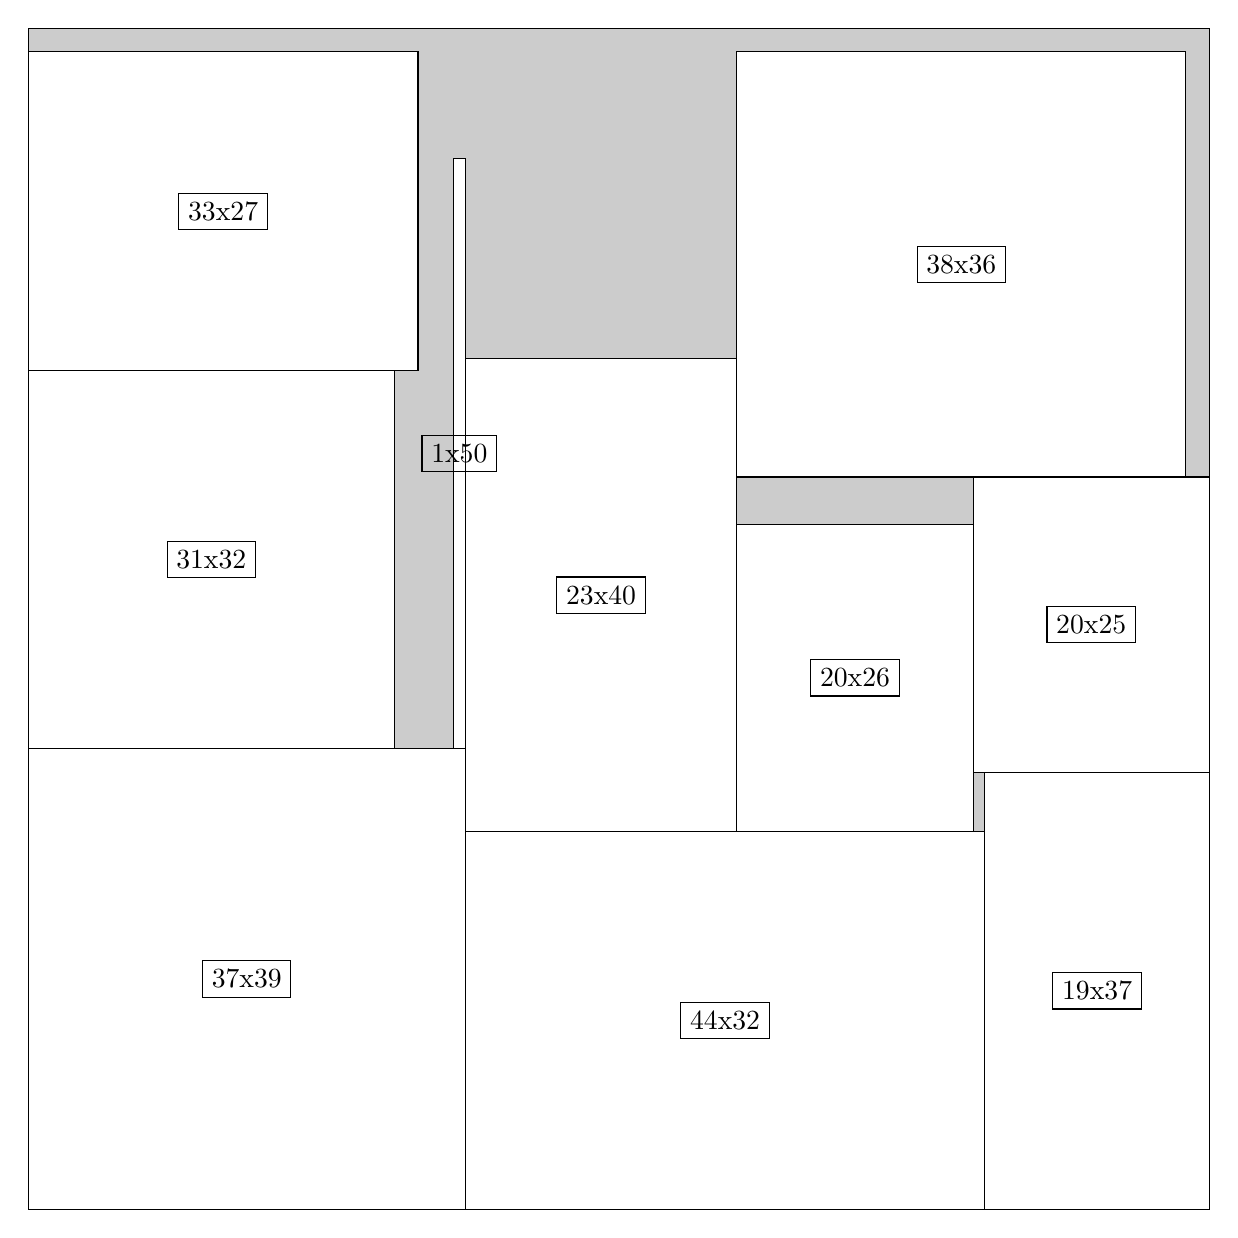
\begin{tikzpicture}[shorten >=1pt,scale=1.0,every node/.style={scale=1.0},->]
\tikzstyle{vertex}=[circle,fill=black!25,minimum size=14pt,inner sep=0pt]
\filldraw[fill=gray!40!white, draw=black] (0,0) rectangle (15.0,15.0);
\foreach \name/\x/\y/\w/\h in {37x39/0.0/0.0/5.55/5.85,44x32/5.55/0.0/6.6/4.8,23x40/5.55/4.8/3.4499999999999997/6.0,31x32/0.0/5.85/4.6499999999999995/4.8,38x36/9.0/9.299999999999999/5.7/5.3999999999999995,33x27/0.0/10.65/4.95/4.05,19x37/12.15/0.0/2.85/5.55,20x26/9.0/4.8/3.0/3.9,20x25/12.0/5.55/3.0/3.75,1x50/5.3999999999999995/5.85/0.15/7.5}
\filldraw[fill=white!40!white, draw=black] (\x,\y) rectangle node[draw] (\name) {\name} ++(\w,\h);
\end{tikzpicture}


w =37 , h =39 , x =0 , y =0 , v =1443
\par
w =44 , h =32 , x =37 , y =0 , v =1408
\par
w =23 , h =40 , x =37 , y =32 , v =920
\par
w =31 , h =32 , x =0 , y =39 , v =992
\par
w =38 , h =36 , x =60 , y =62 , v =1368
\par
w =33 , h =27 , x =0 , y =71 , v =891
\par
w =19 , h =37 , x =81 , y =0 , v =703
\par
w =20 , h =26 , x =60 , y =32 , v =520
\par
w =20 , h =25 , x =80 , y =37 , v =500
\par
w =1 , h =50 , x =36 , y =39 , v =50
\par
\newpage


\end{document}